% Your name
\renewcommand{\YRname}{R. Oechslin}

% Your grade/post
\newcommand{\YRgrade}{M2}

% Submission date
\newcommand{\YRdate}{2018.Apr.27}

% Your research theme
\newcommand{\YRtheme}{Haptic Feedback Controller with Palm Pressurization}

% Work plan
\newcommand{\YRplan}{
	\hspace{-4truemm}
	\begin{tabularx}{170truemm}{|p{50truemm}||X|X|X|X|X|X|X|X|X|X|X|X|}
		\hline
		\multicolumn{13}{|c|}{\parbox[c][10truemm][c]{0truemm}{} \large Research theme: \bf \YRtheme} \\
		\hline
		\hline
		\multicolumn{13}{|c|}{\parbox[c][8truemm][c]{0truemm}{} \large \bf --- Research Plan ---} \\
		\hline
		Term \textbackslash Month & 2 & 3 & 4 & 5 & 6 & 7 & 8 & 9 & 10 & 11 & 12 & 1 \\
		\hline
		% For ``Work plan'', do not change above.
		\hline
		Literature review & & & & & & & & & & & & \\
		\shadecells{2-2}
		\hline
		Design PlayStation Controller  & & & & & & & & & & & & \\
		\shadecells{2-3}
		\hline
		Test PlayStation Controller & & & & & & & & & & & & \\
		\shadecells{5-6}
		\hline
		Frequency Response Analysis & & & & & & & & & & & & \\
		\shadecells{5-6}
		\hline
		Design Pilot Controller & & & & & & & & & & & & \\
		\shadecells{4-6}
		\hline
		Test Pilot Controller & & & & & & & & & & & & \\
		\shadecells{6-7}
		\hline
		& & & & & & & & & & & & \\
		%\shadecells{2-10}
		\hline
		Theoretical Analysis & & & & & & & & & & & & \\
		\shadecells{6-7}
		\hline
		Analyze data and compare & & & & & & & & & & & & \\
		\shadecells{7-8}
		\hline
		Write Thesis & & & & & & & & & & & & \\
		\shadecells{8-8}
		\hline
	\end{tabularx}
}

% Main contents of your work
\newcommand{\YRachievement}{
	Control Scheme
	-	Say how I tested the setup, where and how I applied the signal of the wave generator, story with doubling the voltage level due to 50Ohm output impedance (Arduino has practically infinite input impedance, or very high)
	Photoreceptor circuit (revised)
	Testing of the PlayStation controller
	Results of frequency analysis
	-	Short intro on why pseudo infinite stiffness is ok
	-	Explain min and max values of photoreceptor
	-	Showcases of two to three different frequencies and signal following
	-	Explain formula used for finding magnitude and phase (offset)
	-	Calculate order, show theoretical similar transfer function, discuss point with slope in the end, but not really necessary
	
	Discussion
	-	Control scheme and gui
	-	Frequency response function
	
	Conclusion
	Outlook
	
	\section{Introduction}
	This report is the continuation of the first report about the project "Haptic Feedback Controller with Palm Pressurization". The last report has left off with the conclusion that the Arduino had a limited operating frequency and that the gathered data was not reliable enough, since not the whole region of interest in frequency could be covered. First, the idea was to use an mbed and program it to be able to replace the Arduino. However, with a few tricks %TODO explain what I did with prescaler and such
	it was possible to reduce the time of some commands to a minimum to stay at an operating frequency of $1$kHz. \\
	This report explains the setup and states the result for the adapted controller and provides a somewhat short explanation and discussion of the gathered data.
	
	\section{Experiment and Data Gathering}
	The setup can be seen in figure \ref{}. %TODO make reference
	For this experiment, a total of four springs, arranged symmetrical on the palmpad have been used. The springs have a spring constant of $k_s = 1.5$N/mm which corresponds to an equivalent spring constant of $k_{eq} = 6$N/mm. They are distributed around the palm pad, where in their middle the photoreceptor has been attached, to measure the distance between the L-plate and the palm pad. It therefore measures the compression of the springs, which can be related to the output force by Hooke's law as:
	\begin{equation}
		F = k_{eq}x 	
	\end{equation}
	
	\subsection{Setup}
	In this experiment a thorough frequency response analysis shall be done on the controller. On the left-hand side the motor with a reduction ratio of $33:1$ has been used, whereas for the right-hand side, the motor has a reduction ratio of $112:1$. \\
	A reference signal is fed into the Arduino, which then controls the motors to match the compression of the springs with the reference. The operational distance of the photoreceptor to the palm pads is $2$ to $4$mm which lies within the more sensitive region of the sensor.
	
	\subsection{Control Scheme}
	The reference signal is given by the Function Generator SG-4115. This generator has an intrinsic output impedance of $50$Ohm. This means, that it expects to have a device connected to it with the same value as input impedance. If this is the case, these two elements form a simple voltage divider and only half of the voltage is applied to the target device. However, this is not the case for the Arduino, since it has a considerably higher input impedance. Therefore, the settings made on the function generator result in double the voltage on the Arduino. From this point on, this issue shall be neglected and all future voltage indications refer to the voltage level as seen by the Arduino.\\
	The function generator produces a sine wave between $0$ and $5$V with a frequency ranging from $1$ to $100$Hz. The Arduino reads this voltage and controls the motor to have a proportional spring compression accordingly. In this case $0$V as reference signal is $0\%$ compression and $5$V corresponds to $100\%$ compression. The control scheme of this setup can be seen in figure \ref{fig:frf_measure_points}.
	\begin{figure}[h!]
		\centering
		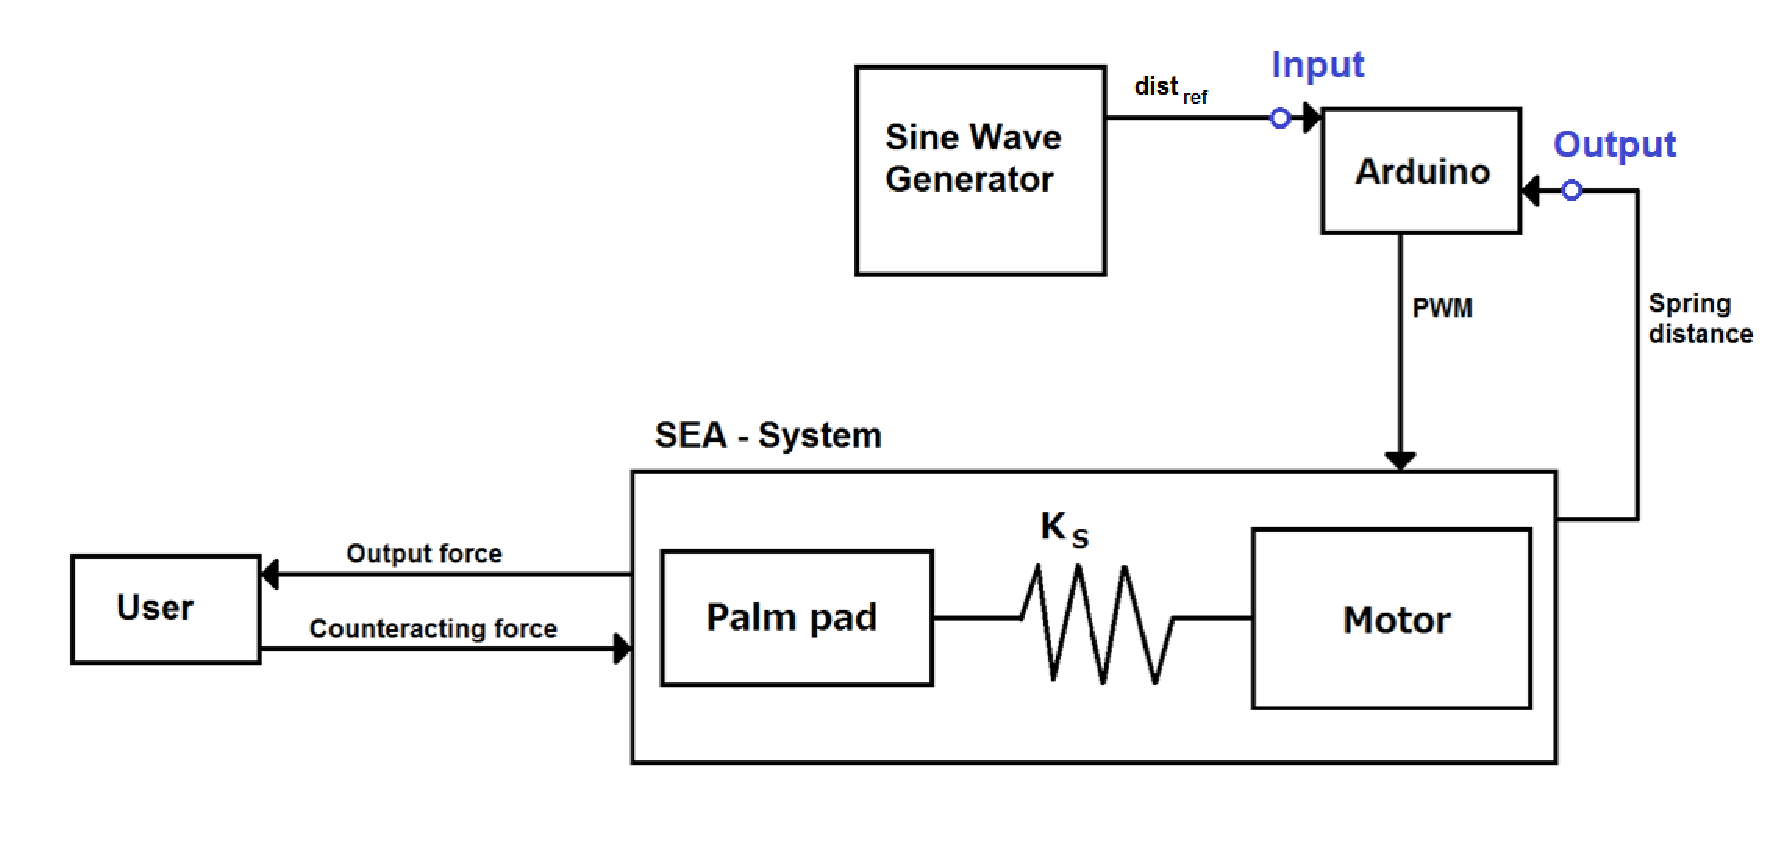
\includegraphics[width=0.6\linewidth]{Figs/frf_measure_points}
		\caption{Control scheme for the frequency response analysis.}
		\label{fig:frf_measure_points}
	\end{figure}
	In this case the output force from the user is infinite, since the palm pads have been blocked by a wall.
	
	\subsection{Photoreceptor Circuit}
	The circuit of the photoreceptor can be found in figure \ref{fig:tpr105_circuit}. The components chosen are the TPR-105 for the sensor, $R_1 = 330\Omega$ and $R_2 = 27k\Omega$.
	
	\begin{figure}[h!]
		\centering
		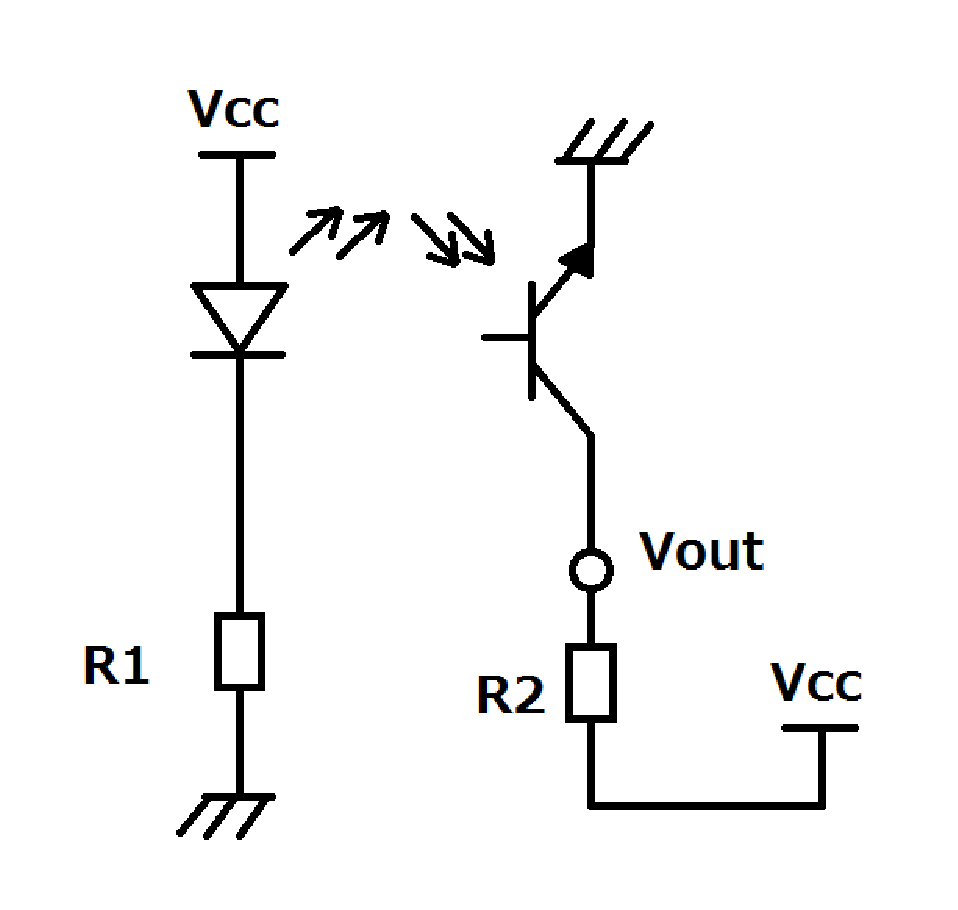
\includegraphics[width=0.2\linewidth]{Figs/tpr105_circuit}
		\caption{Photoreceptor circuit.}
		\label{fig:tpr105_circuit}
	\end{figure}
	The photoreceptors working principle is based on detecting the amount of reflected light. This controls the base current $i_B$ of the transistor in the schematic. This base current then determines the collector current $i_C$. Specific to this setup, the distance and therefore the output force controls the amount of light that is reflected on the wall of the palm pad. Therefore, we have:
	\begin{equation}
	F_{output} = k_{eq} \Delta x \propto i_B
	\end{equation}
	\begin{equation}
	i_C = h_{FE} i_B
	\end{equation}
	\begin{equation}
	V_{out} = V_{CC} - h_{FE} R_2 i_C = V_{CC} - K R_2 \Delta x
	\end{equation}
	Where $h_{FE}$ is the forward current gain and $K$ is a constant given by $h_{FE} k_{eq}$.
	
	The two resistor values have been empirically found to have the highest sensitivity but not saturating the measurement. The sensitivity decreases with a smaller resistor, since at a certain point, the Arduino cannot detect a change in voltage anymore. Saturation occurs, when the value of $R_2$ is too high.
	
	\subsection{Identification of Operational Range (Photoreceptor)}
	To find the receptor values at maximum compression of the springs, a simple test has been made, where one time $0$V has been applied to the motors, and another time $20$V has been applied. This $20$V value is within a safety margin of the maximum applicable voltage given by the datasheet of the motors. The result can be seen in the figure \ref{fig:max_volt_applied_plot}.
	
	\begin{figure}[h!]
		\centering
		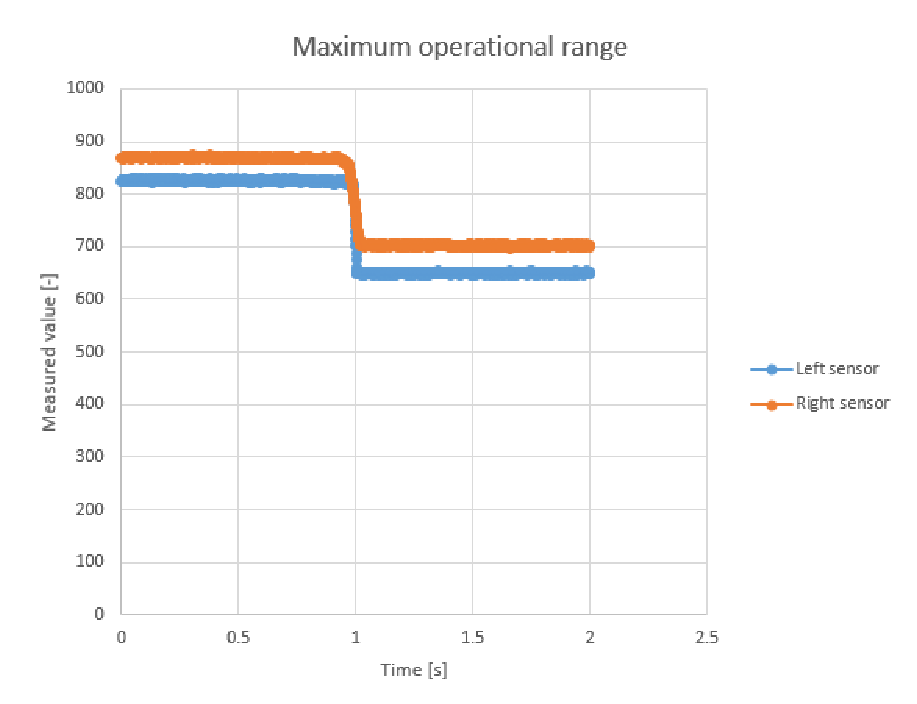
\includegraphics[width=0.6\linewidth]{Figs/max_volt_applied_plot}
		\caption{Operational range of photoreceptor with springs at rest and in full compression.}
		\label{fig:max_volt_applied_plot}
	\end{figure}
	
	The values that have been found to be the limiting values are resumed in table \ref{tab:oper_range}.
	
	\begin{figure}[h!]
		\centering
		\begin{tabular}{|l|c|c|c|c|c|}
			\hline
			& Sensor reading & Distance & Sensor reading & Distance & Max output  \\
			& MAX (rest) & (rest) & MIN (compression) & (compression) & force \\ \hline \hline
			Left side & 830 & 2.35mm & 650 & 4mm & 9.9N \\ \hline
			Right side & 870 &2.2mm & 700 & 4mm & 10.8N \\ \hline
		\end{tabular}
		\caption{Identified operational range}
		\label{tab:oper_range}
	\end{figure}
	
	Having found these two values, the photoreceptor measurements can be mapped to this range with an 8-bit value. This means that $0$ is no compression and $255$ is fully achievable compression.
	
	\section{Frequency Response Analysis}
	To conduct the frequency response analysis in a meaningful environment, the controller has to be tested under conditions close to the operational ones. To be able to control the distance between palm pads L-plates, and therefore the compression ratio of the springs, the palm pads have been blocked mechanically. With the wave generator producing the reference signal, the Arduino controlled the motors to match the compression with the reference. Figure \ref{} shows some testcases.
	
	%TODO put pictures from data_analysis 1Hz, 12.6Hz and 100Hz.
	\begin{figure}[h!]
		\centering
		\includegraphics[width=0.6\linewidth]{Figs/}
		\caption{.}
		\label{fig:}
	\end{figure}
	With these signals one can calculate the amplification factor between the reference signal and the output signal, as well as the phase shift.
	
	\subsection{Sinewave Fitting}
	As described in this example\cite{exnumerus2010}, one can fit a sinewave with the linear least square method to the samples. This function returns the phase, amplitude and the bias. In this case, the difference in phase between input and output, as well as the amplitude ratio is needed in order to plot a Bode diagram.
	
	\subsection{Bode Diagram}
	The results of the frequency response analysis are shown in figure \ref{}.
	


	
	%�����܂�
}


